\section{Statistisk baggrund}

\subsection{Randomiseret eksperiment}
Vi bruger følgende terminologi:
\begin{itemize}
	\item Sample space: Mængde $\Omega$ af alle udfald
	\item Elementary events: Elementer i $\Omega$. Hvert eneste element har en tilknyttet sandsynlighed
	\item Event: Delmængde $\E$ af $\Omega$
\end{itemize}

Lad os tage et eksempel med 4 møntkast. Da vil der være $2^4 = 16$ elementary events i $\Omega$ med sandsynlighed $1/16$ hver.


\begin{figure}[H]
	\centering
	\begin{subfigure}[b]{0.23\textwidth}
		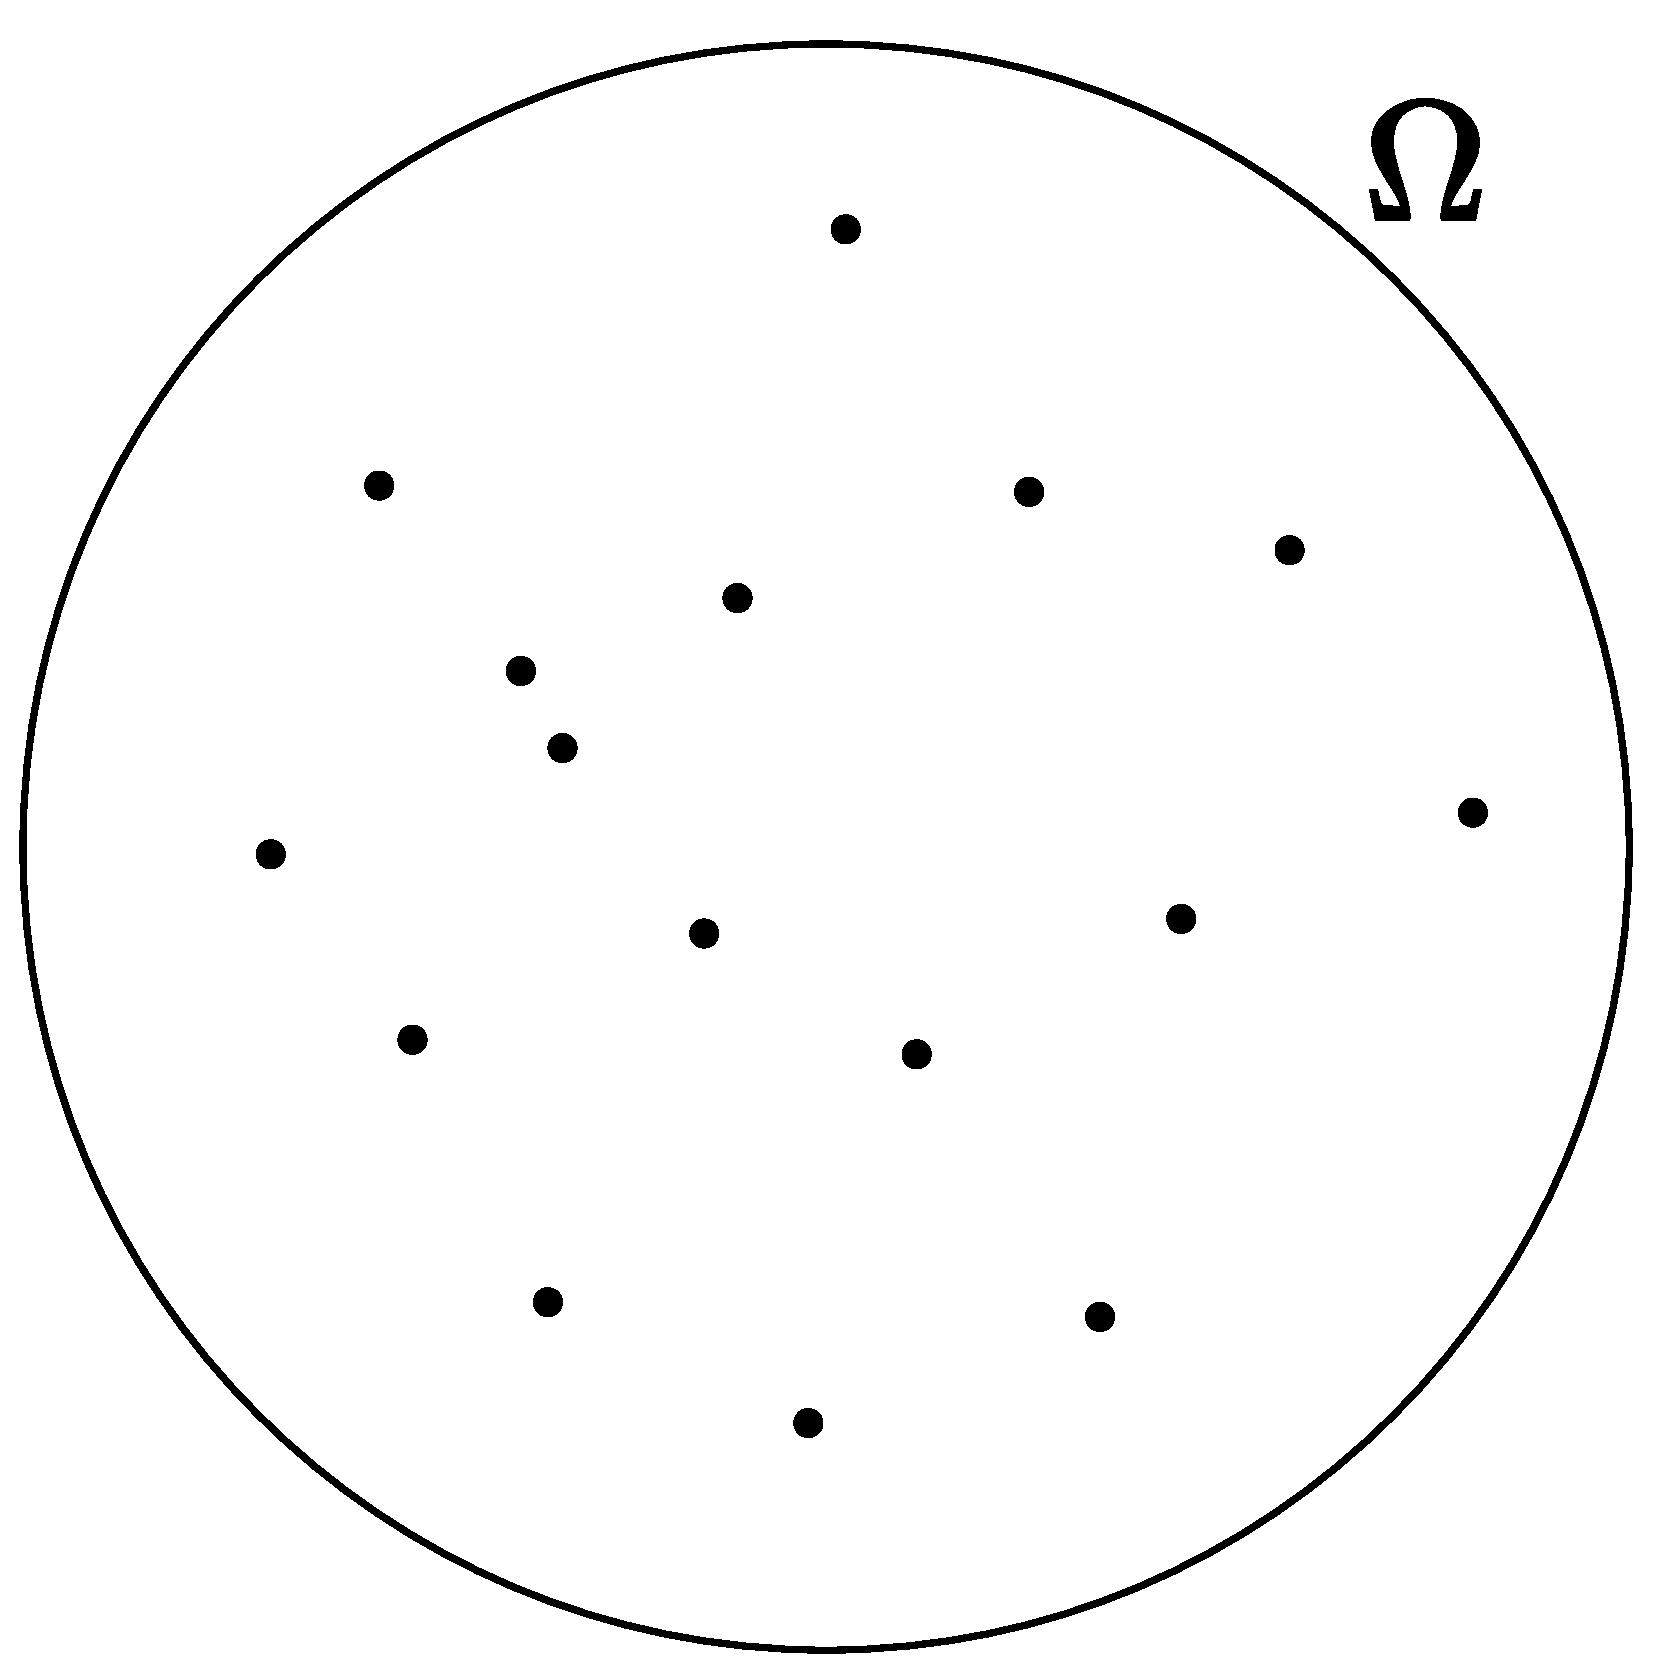
\includegraphics[width=\textwidth]{elem-events.pdf}
		\caption{Et udfaldsrum $\Omega$ med 16 elementary events.}
		\label{fig:elem}
	\end{subfigure}
	~
	\begin{subfigure}[b]{0.23\textwidth}
		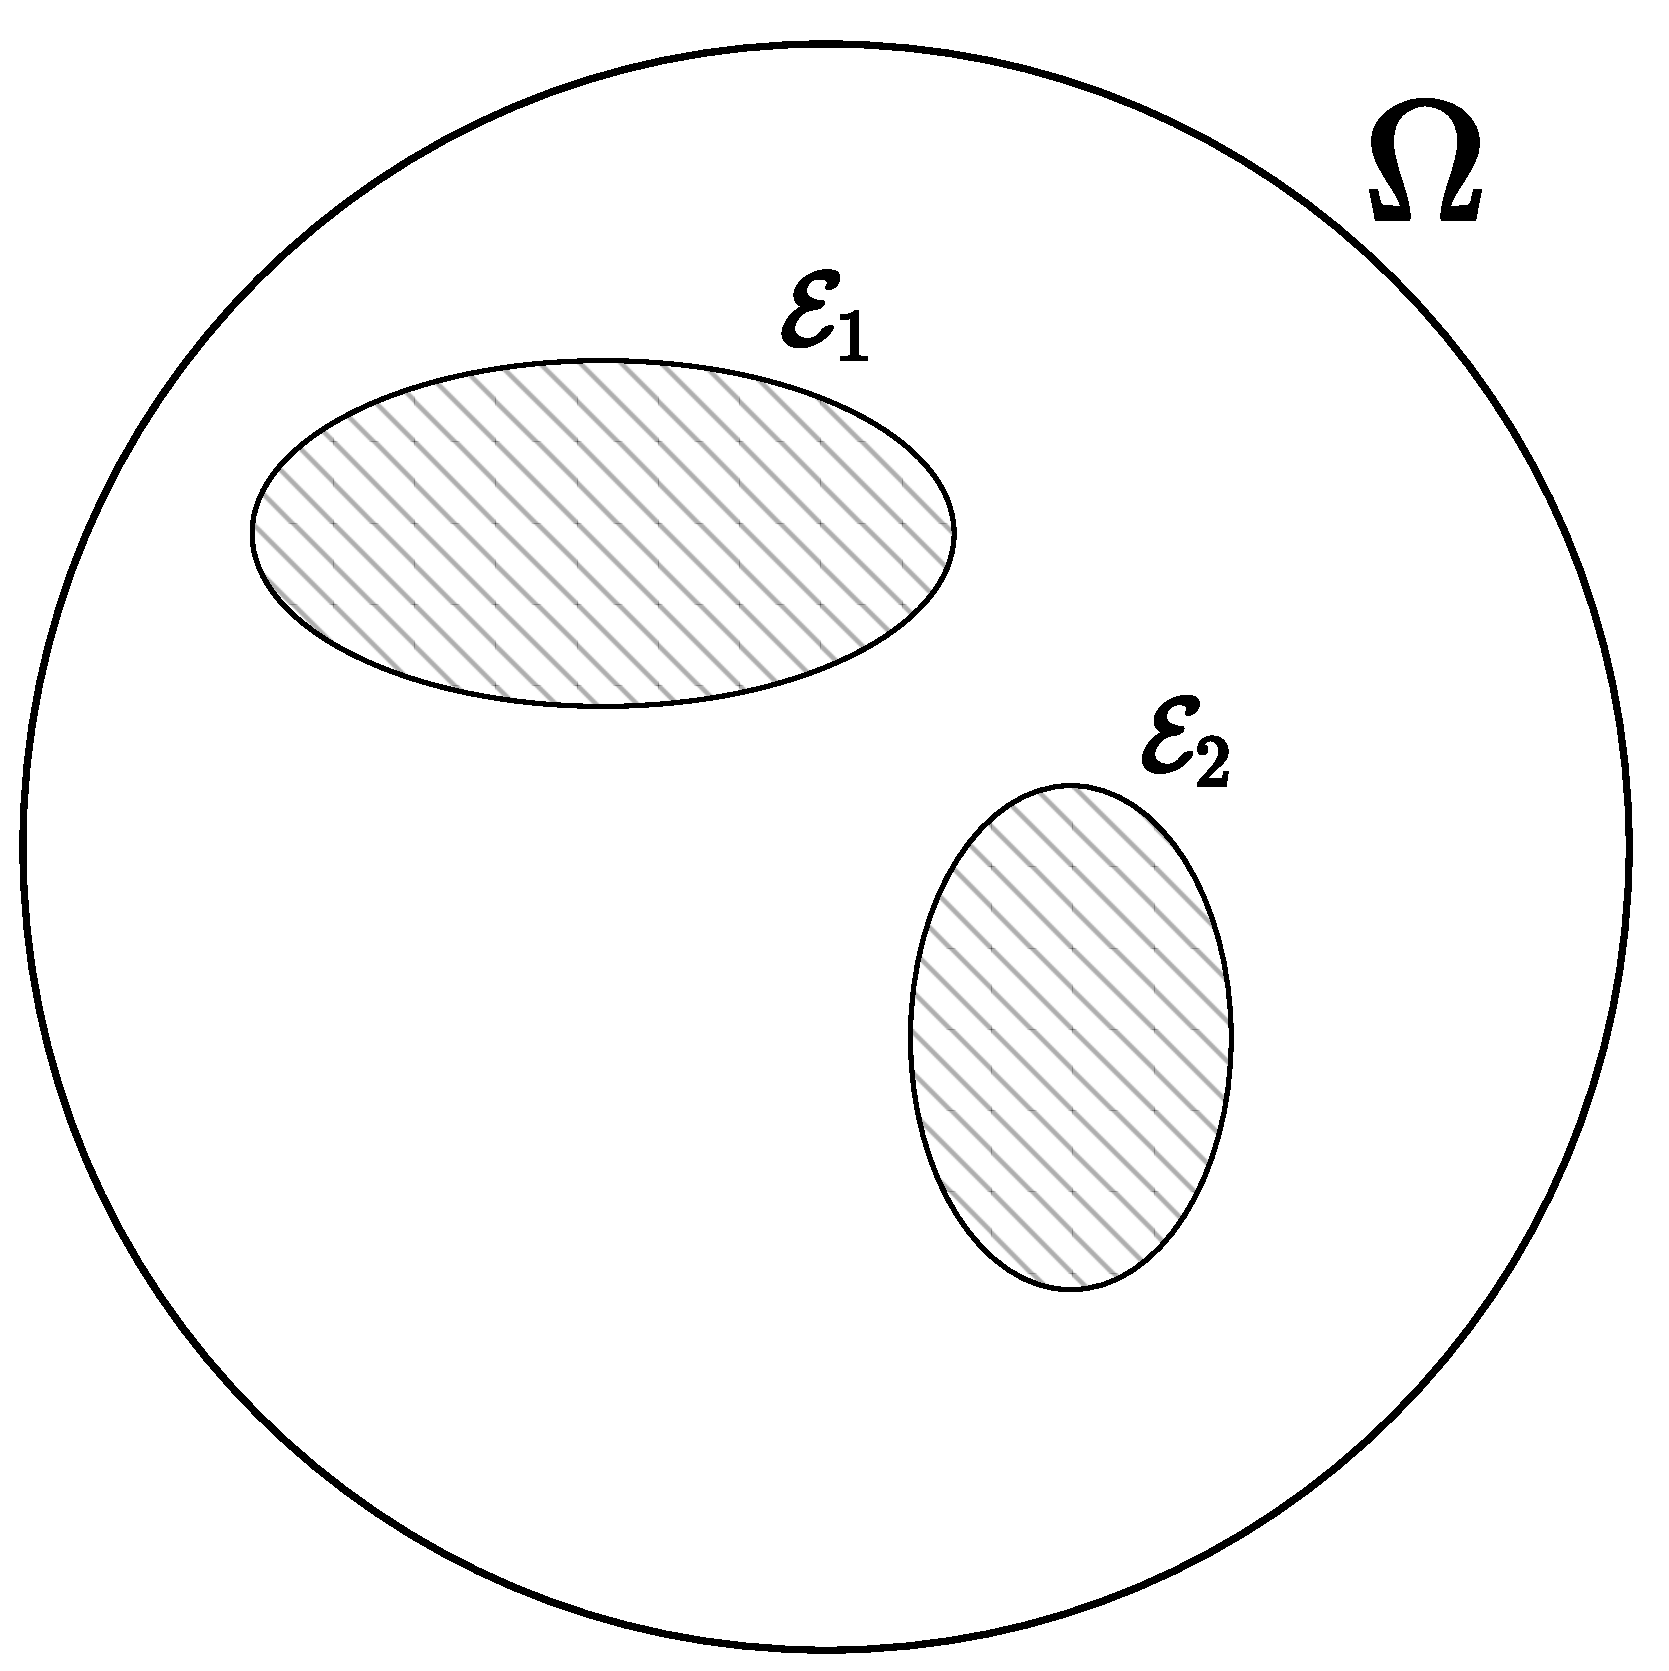
\includegraphics[width=\textwidth]{disjunkt.pdf}
		\caption{To disjunkte events. $\P[\E_1 \cup \E_2]$ skraveret.}
		\label{fig:disjunkt}
	\end{subfigure}
	~
	\begin{subfigure}[b]{0.23\textwidth}
		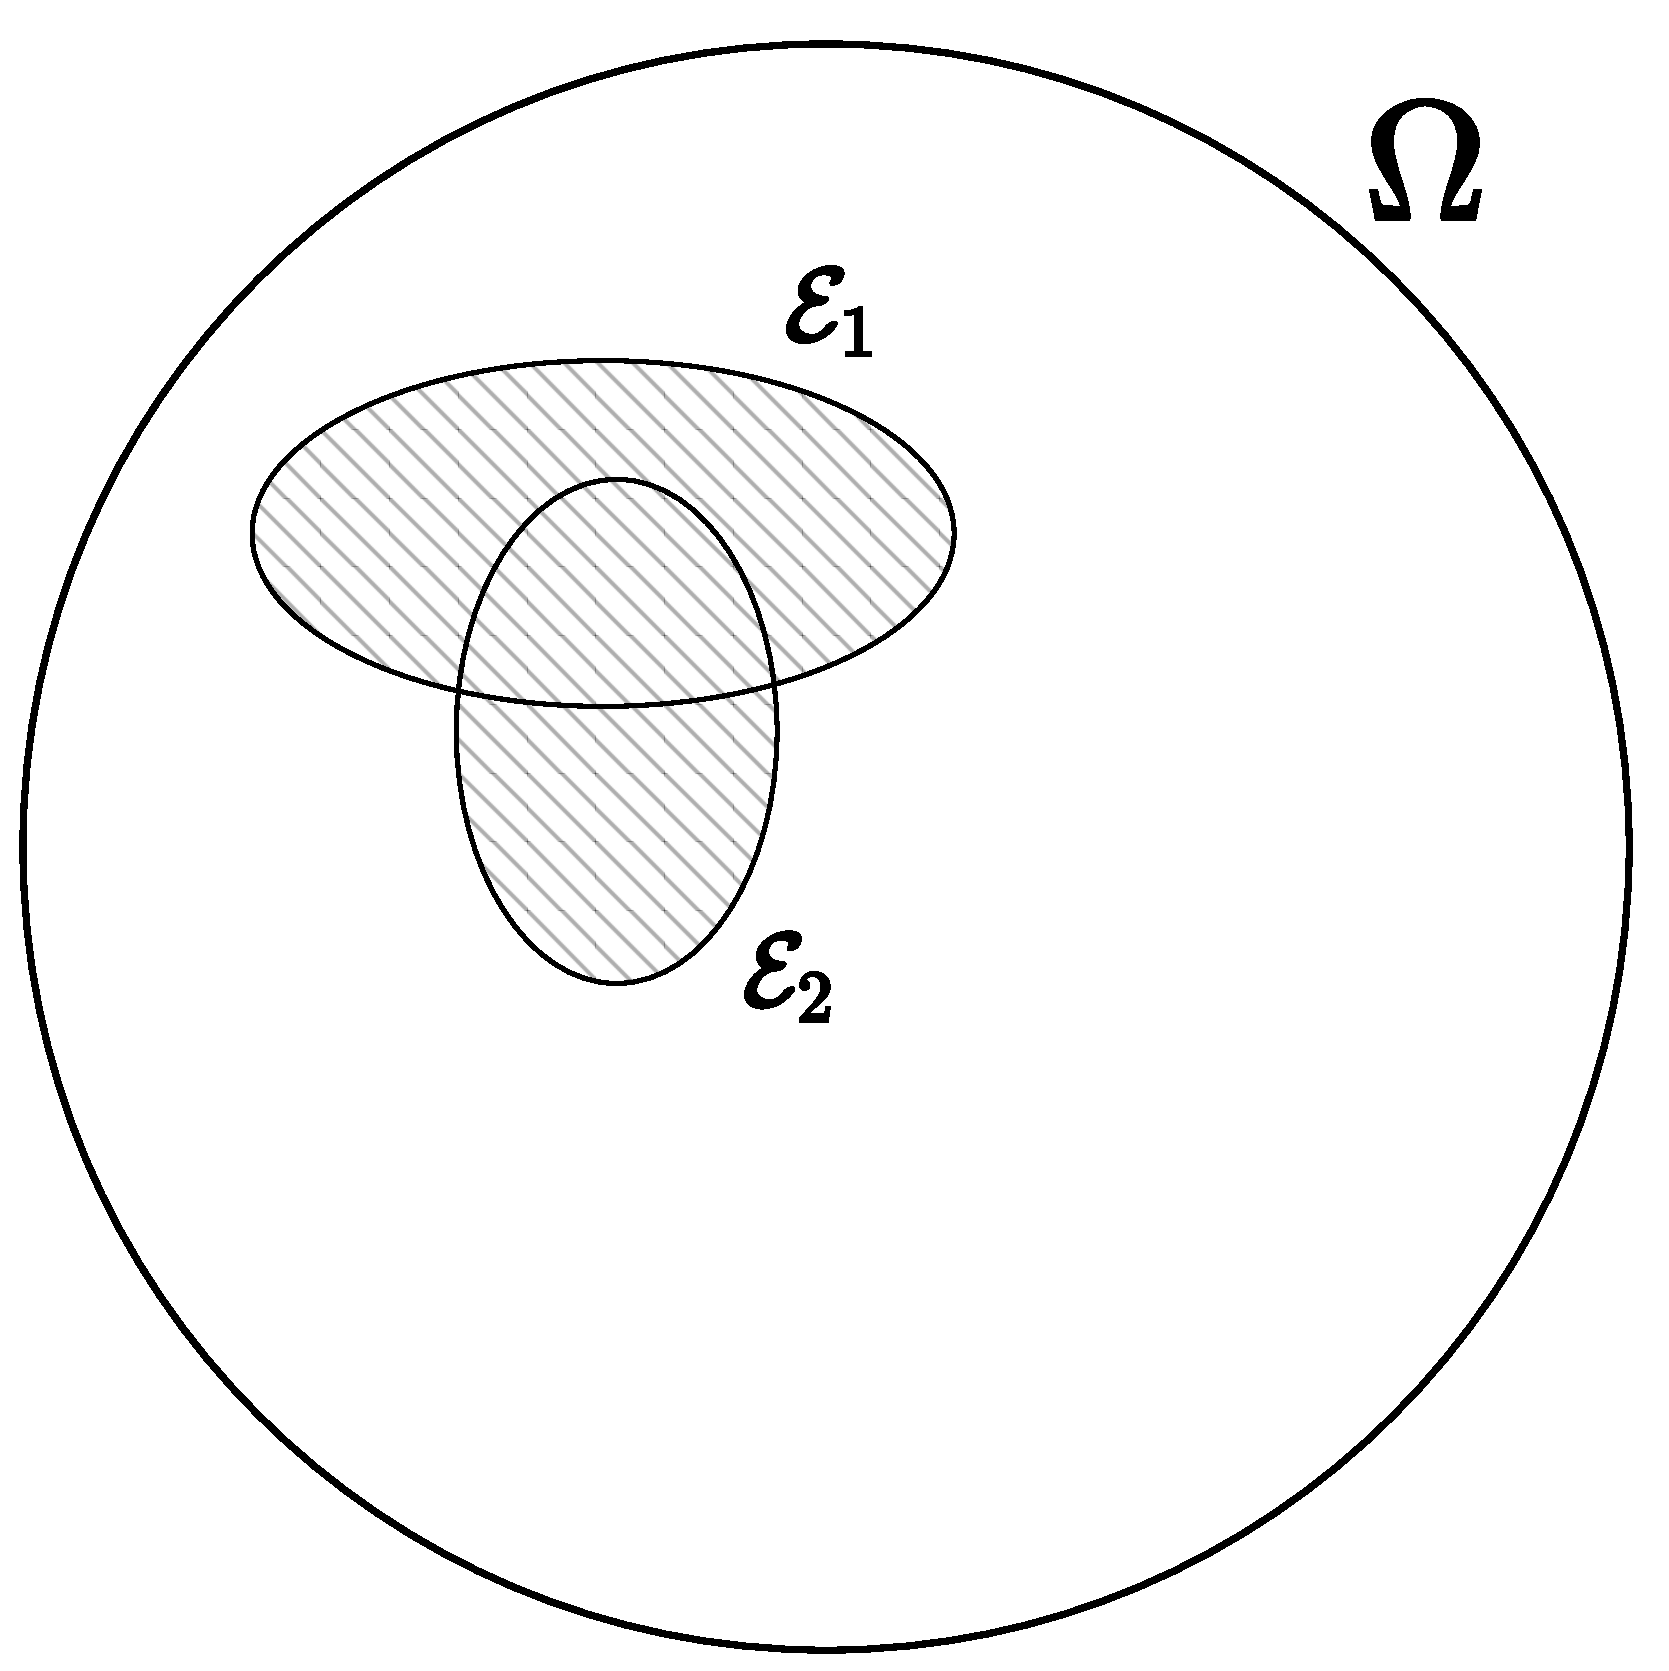
\includegraphics[width=\textwidth]{union.pdf}
		\caption{To events der overlapper. $\P[\E_1 \cup \E_2]$ skraveret.}
		\label{fig:union}
	\end{subfigure}
	~
	\begin{subfigure}[b]{0.23\textwidth}
		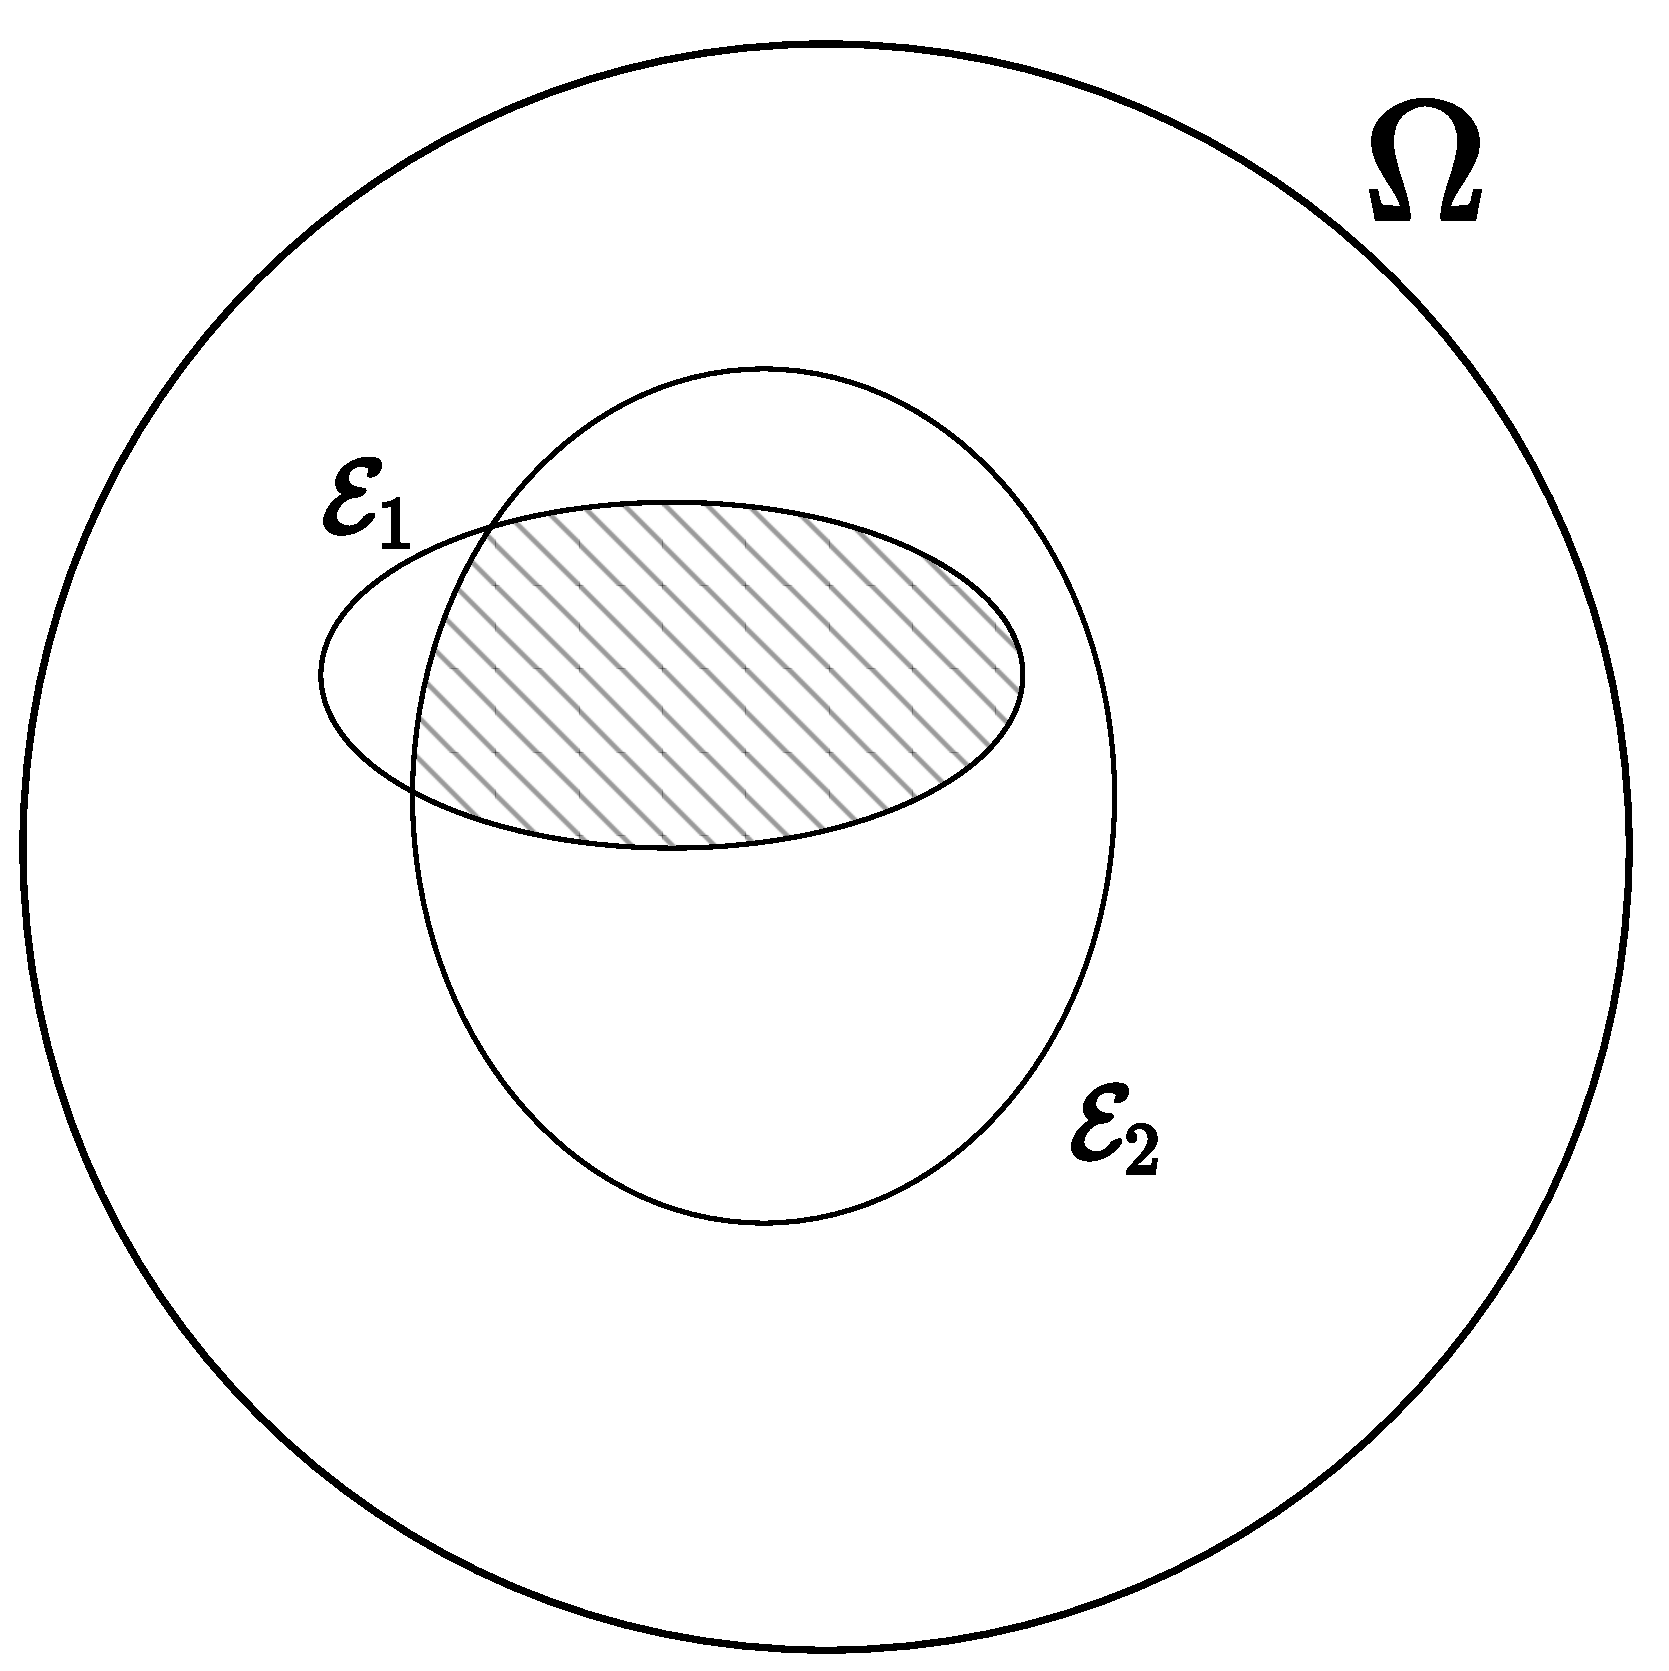
\includegraphics[width=\textwidth]{conditional.pdf}
		\caption{To events der overlapper. $\P[\E_1 \cap \E_2]$ skraveret.}
		\label{fig:conditional}
	\end{subfigure}
	\caption{En række forskellige fænomener i et udfaldsrum $\Omega$}
	\label{fig:sample-spaces}
\end{figure}


Så kunne vi f.eks. have at et event $\E$ er mængden af elementary events med $\geq 3$ heads:
\begin{align*}
\E &= \curly{HHHT, \ HHTH, \ HTHH, \ THHH, \ HHHH}\\
\P[\E] &= \frac{5}{16}
\end{align*}

Givet parvis disjunkte events $\E_1, \cdots, \E_n$, har vi følgende, som svarer til det skraverede område på \ref{fig:disjunkt}:
\begin{align} \label{eq:disjunkt}
\P[\E_1 \cup \cdots \cup \E_n] = \P \square{\bigcup_{i=1}^n \E_i} = \sum_{i=1}^{n} \P[\E_i]
\end{align}

\subsubsection{Union bound}
Mere generelt kan ovenstående formuleres som, at givet events $\E_1, \cdots, \E_n$ (som ikke nødvendigvis er disjunkte), så vil følgende gælde, hvor venstresiden svarer til det skraverede område på \ref{fig:union}:
\begin{align} \label{eq:union-bound}
\P \square{\bigcup_{i=1}^n \E_i} \leq \sum_{i=1}^{n} \P[\E_i]
\end{align}

\subsubsection{Conditional probability}
Givet to events $\E_1$ og $\E_2$, så vil sandsynligheden af $\E_1$ givet $\E_2$ kunne beregnes som:
\begin{align}
\P \square{\E_1 | \E_2} = \frac{\P[\E_1 \cap \E_2]}{\P[\E_2]}
\end{align}
hvor $\P[\E_1 \cap \E_2]$ er sandsynligheden for at begge events sker. På \ref{fig:conditional} svarer dette til det skraverede område divideret med hele området for $\E_2$. På samme måde vil $\P[\E_2 | \E_1]$ være det skraverede område divideret med hele området for $\E_1$.\\

Eksempelvis kunne vi have følgende:
\begin{align*}
\E_1 &= \curly{HHHH}       &\P[\E_1 | \E_2] &= 1/2\\
\E_2 &= \curly{HHHH, HHHT} &\P[\E_2 | \E_1] &= 1
\end{align*}

\subsection{Stokastiske variable (random variables)}
En random variable er en funktion $X: \Omega \rightarrow \R$:

Eks. med to møntkast:
\begin{itemize}
	\item HH: 2 kr i fortjeneste
	\item HT: 0 kr
	\item TH: 0 kr
	\item TT: -1 kr
\end{itemize}

$X$ udtrykker fortjenesten. $X = 2$ hvis HH osv.\\

Indicator variabel: Random variabel med værdier i $\{0, 1\}$.

\subsubsection{Expectation af $X$, $\e[X]$}
\begin{align} \label{eq:exp-random}
\e[X] = \sum_{x} x \, \P[X = x]
\end{align}

For vores ovenstående eksperiment vil det f.eks. være:
\begin{align*}
\e [X] &= 2 * \P[X = 2] + 0 * \P[X=0] + (-1) * \P[X = -1]\\
       &= 2 * \frac{1}{4} - 1 * \frac{1}{4}\\
       &= \frac{1}{4}
\end{align*}


\subsubsection{Linearity of expectation}
Givet random variables $X_1, \cdots, X_n$ og givet konstanter $c_1, \cdots, c_n$, så vil
\begin{align} \label{eq:linearity}
\e \square{\sum_{i=1}^{n} c_i X_i} = \sum_{i=1}^n c_i \e[X_i]
\end{align}

\subsubsection{Probability distribution function (pdf)}
Vi kan opskrive en probability distribution function for $X$. Nedenfor ses det plottet. Af de to typer til højre ønsker vi oftere en af typen $\e[Y]$, da vi så er mere sikre på hvad vi vil få:
\begin{figure}[H]
	\begin{center}
		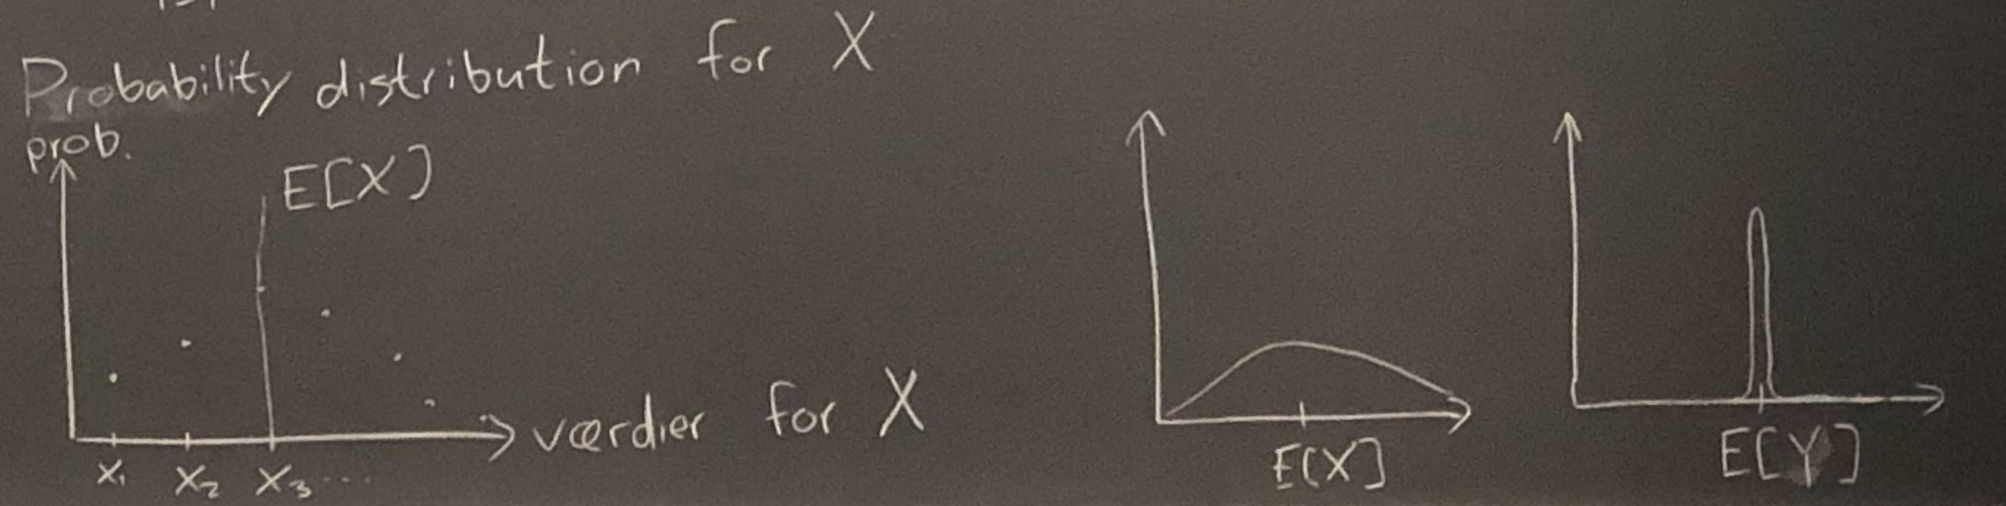
\includegraphics[width=\textwidth]{pdf.png}
	\end{center}
	\caption{Probability distribution function}
	\label{fig:pdf}
\end{figure}

\subsection{Bernoulli distribution}
Lad os nu sige at vi med et enkelt møntkast ikke har sandsynligheder $1/2$ for hvert udfald, men i stedet at $\P[H] = p$ og $\P[T] = 1-p$.

Lad da $X$ være en indikator-variabel, som er 1 ved $H$ og 0 ved $T$.

Da vil:
\begin{align*}
\P[X = 1] &= p\\
\P[X = 0] &= 1 - p\\
    \e[X] &= \P[X = 1] = p
\end{align*}
